Alternative text, or `Alt text', is a textual description of an equation, link or figure that can be used to replace the visual information in that element. This is often seen as a text `pop-up' in PDF readers. %For example, passing the pointer over the following equation should reveal a pop-up:

\begin{equation}
%\pdftooltip{a^2+b^2=c^2}{An equation}
a^2+b^2=c^2
\end{equation}

Alt text can be added after the PDF is compiled using a PDF editor such as Adobe's Acrobat Pro.

Alternatively -- and probably best for ensuring that the final document is what the author intended -- it can be generated from within the source document using the \texttt{pdftooltip} environment from the \texttt{pdfcomment} package. For example, it could be added to
 the previous equation using \verb?\pdftooltip{a^2+b^2=c^2}{An equation}?.

The same approach can be used to create alt text for images. The general form is \verb?{\pdftooltip{\includegraphics[config]{path}}{alt-text}}?.

% For example, Figure \ref{fig:NRELimagesWithAltText} has been labeled with a tool tip. 
%
% \begin{figure*}
% 	\centering
%         \begin{subfigure}[t]{.45\linewidth}
% 		\centering
% 		{\pdftooltip{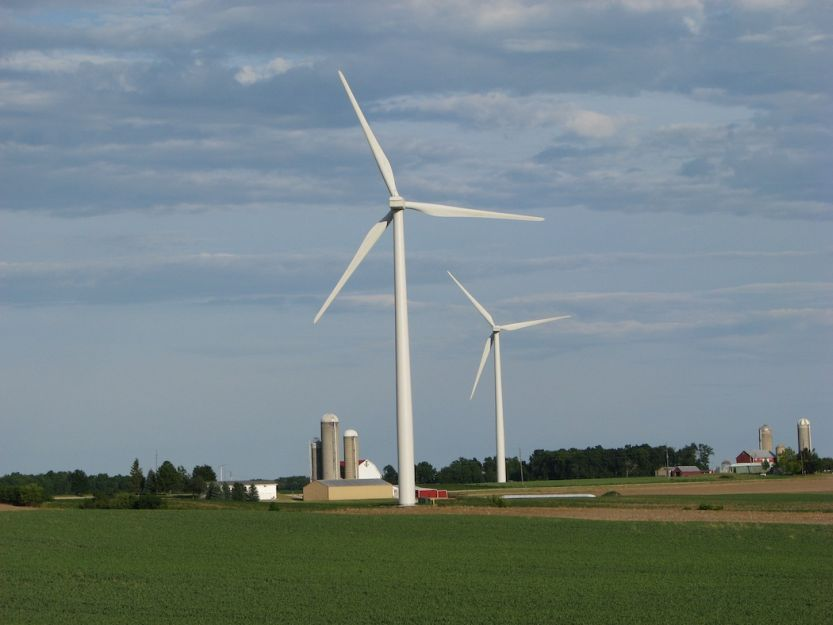
\includegraphics[height=2in]{../common_files/21206.jpg}}{Wind turbines at the Forward Wind Energy Center in Fond du Lac and Dodge Counties, Wisconsin. (Photo by Ruth Baranowski / NREL)}}
% 		\caption{Wind turbines at the Forward Wind Energy Center in Fond du Lac and Dodge Counties, Wisconsin. (Photo by Ruth Baranowski / NREL)}\label{fig:21206WithAltText}
% 	\end{subfigure}%
%         \hfill
%         \begin{subfigure}[t]{.45\linewidth}
% 		\centering
% 		{\pdftooltip{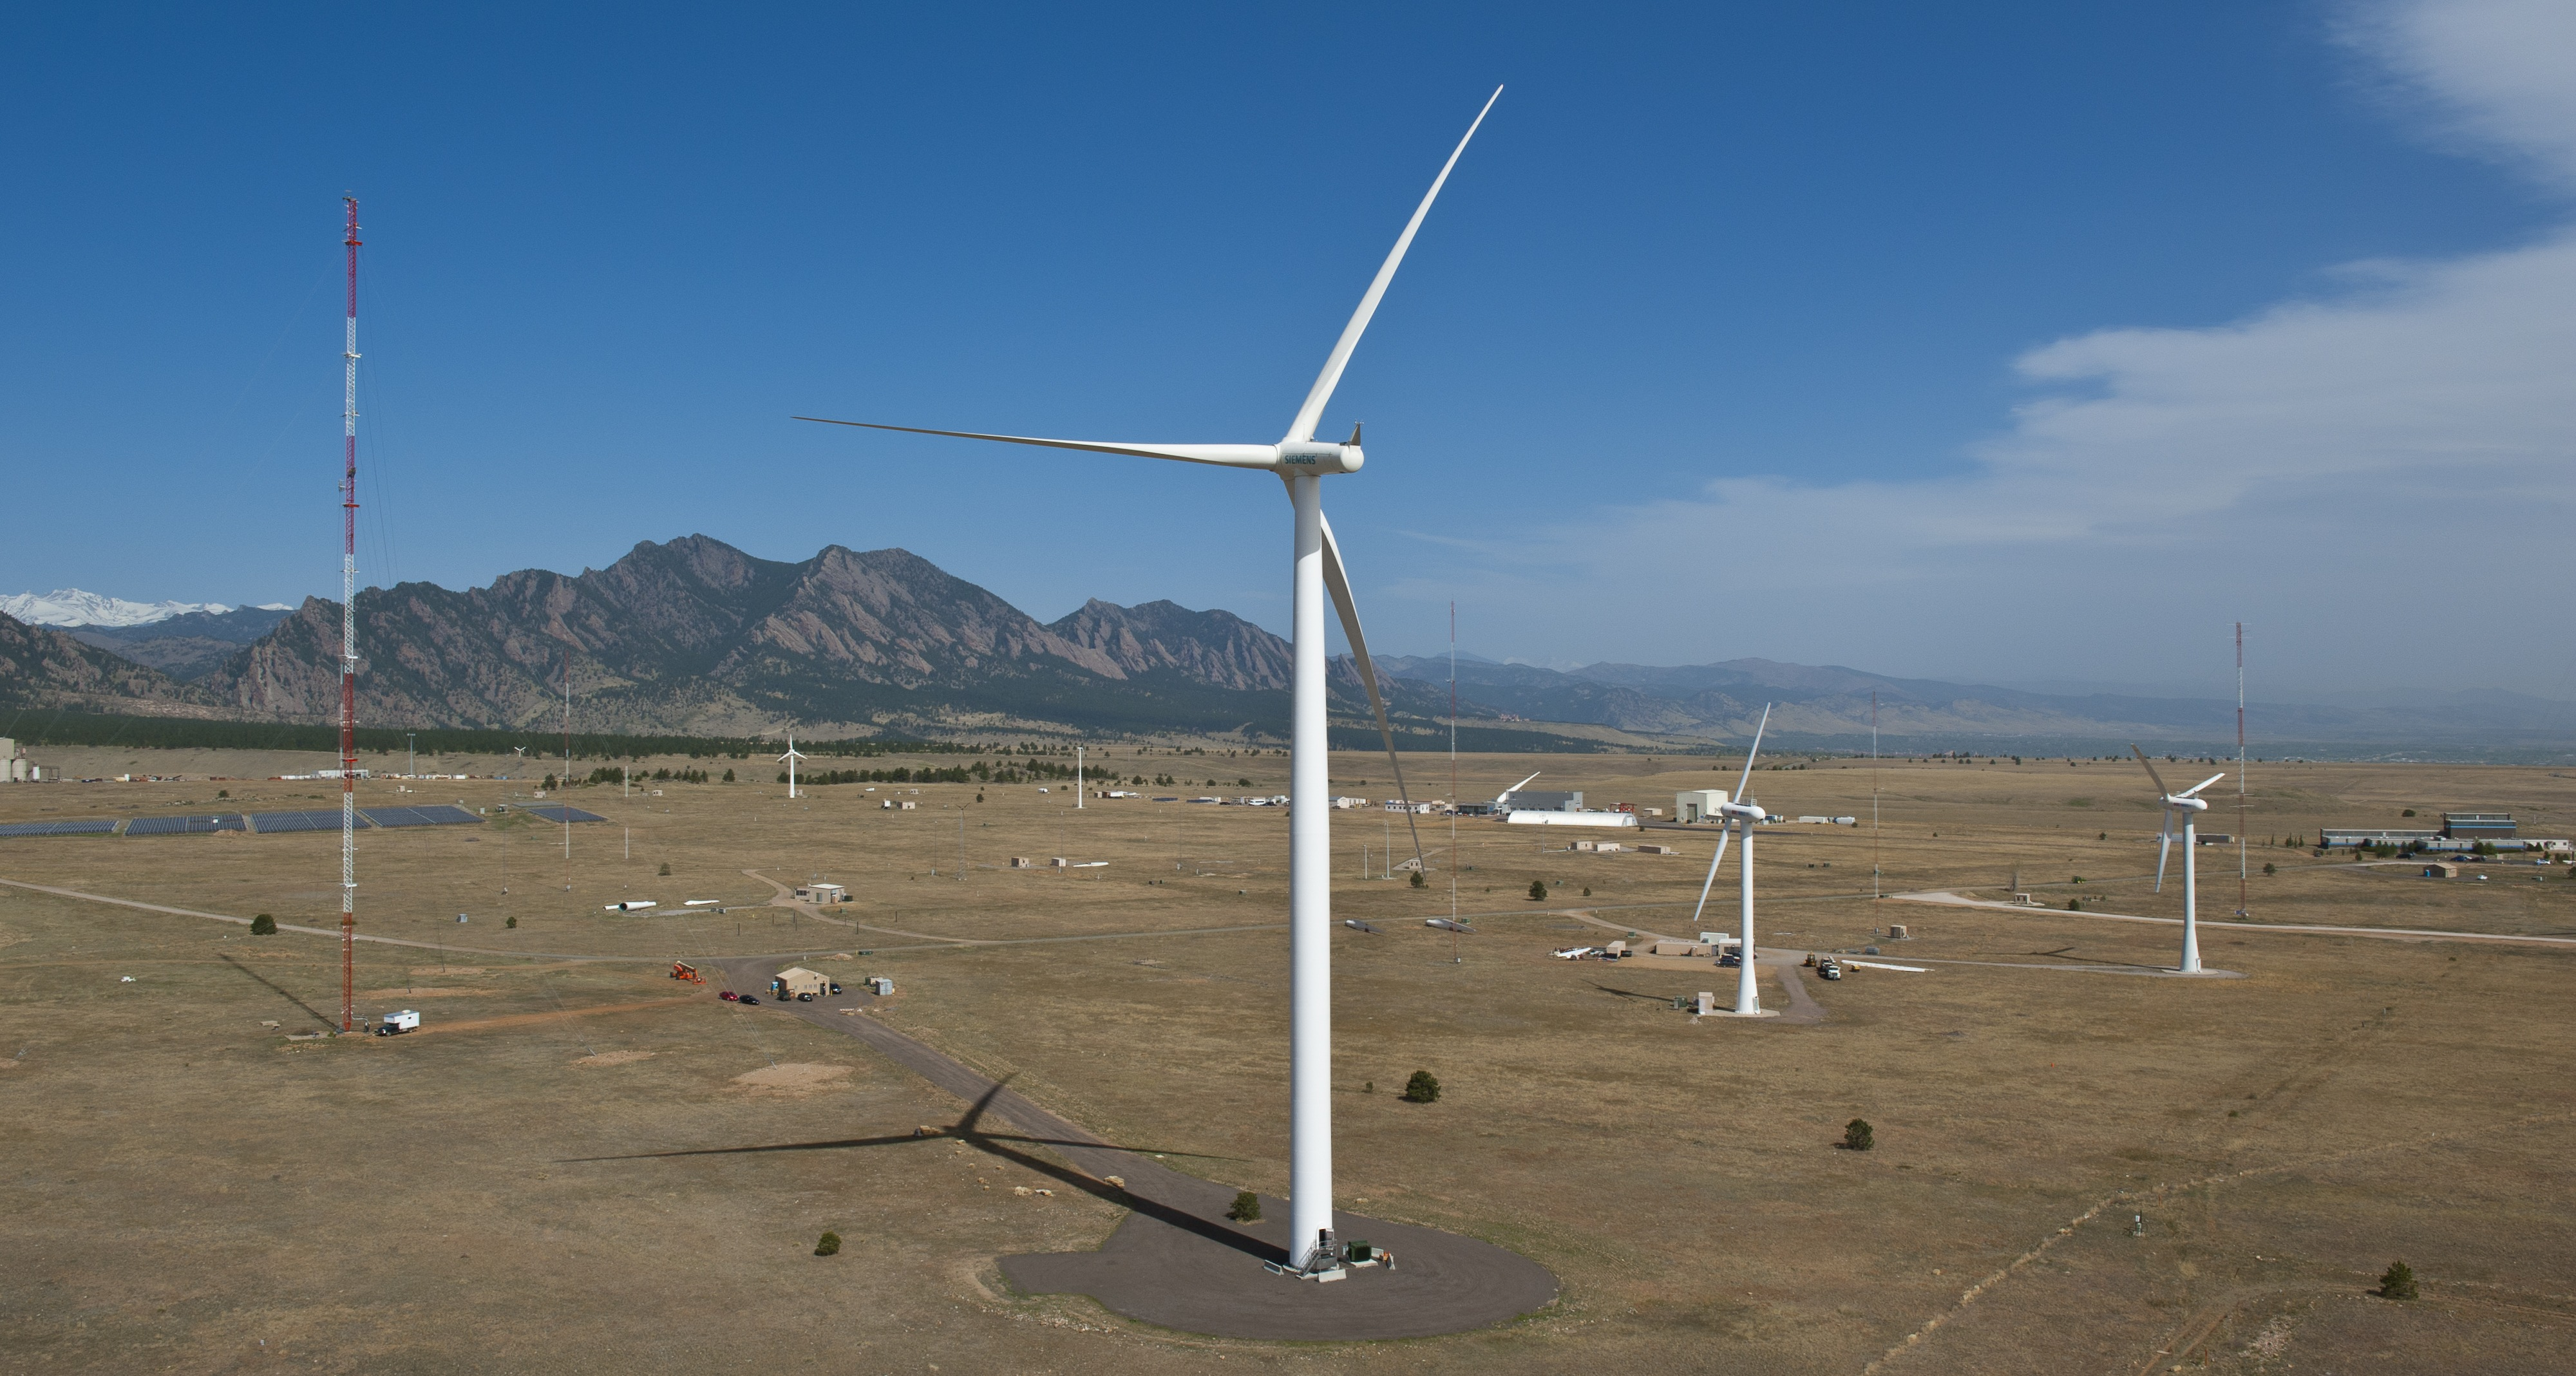
\includegraphics[height=2in]{../common_files/20018.jpg}}{Aerial view of the National Wind Technology Center. (Photo by Dennis Schroeder / NREL)}}
% 		\caption{Aerial view of the National Wind Technology Center. (Photo by Dennis Schroeder / NREL)}\label{fig:20018WithAltText}
% 	\end{subfigure}
% 	\caption{Images with Alt Text}\label{fig:NRELimagesWithAltText}
% \end{figure*}